\chapter{Breadboard Prototype}
\label{cap:breadboardPrototype}

The first phase of developing the new clocking device involved thorough research into available components and 
microcontrollers in the market. Factors such as cost, functionality, and potential drawbacks were carefully 
evaluated to inform the selection process. Subsequently, selected components were tested by constructing a 
basic prototype on a breadboard to assess functionality and performance. Demonstrating the viability of the 
project at this stage was crucial for ensuring its continued development and success.

\section{Hardware selection}

Firstly, considering that the development was urgent, it would only be possible to use an already made 
controller. There were two routes to take:
\begin{itemize}
	\item Using a \textbf{single-board computer}.
	\item Using a \textbf{microcontroller}.
\end{itemize}

The team's familiarity with \textit{Raspberry Pi} products and their reputation for reliability led to the 
decision to utilize their offerings for the project. Given the lightweight processing requirements, the 
\textit{Raspberry Pi Zero 2 W}, a cost-effective single-board computer with built-in WiFi capabilities, emerged 
as a suitable option. Alternatively, the \textit{Raspberry Pi Pico W}, a microcontroller, presented another 
viable choice.

However, it's important to note that while the \textit{Pi Zero} offers more features and functionality, it 
comes at a higher cost compared to the \textit{Pi Pico}. In fact, it costs almost three times as much. 
Therefore, careful consideration is warranted to determine whether the additional expense justifies the benefits.

\begin{figure}[h]
    \centering
    \begin{minipage}[b]{0.45\textwidth}
        \centering
        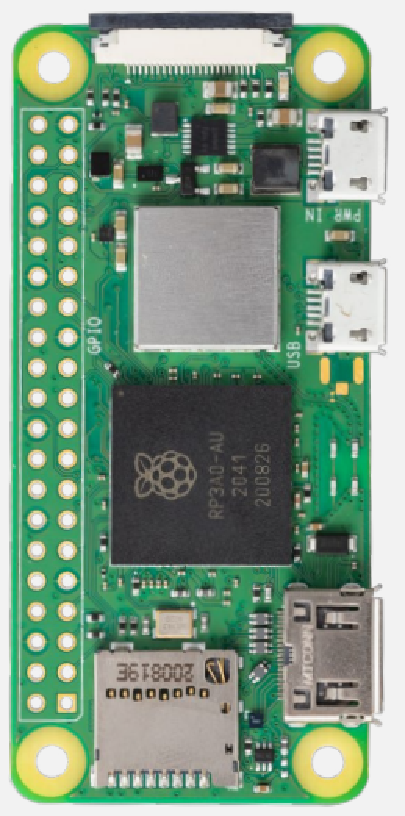
\includegraphics[width=.6\textwidth]{Imagenes/Vectorial/piZero2W.pdf}
        \caption{Raspberry Pi Zero 2 W}
        \label{fig:piZero2W}
    \end{minipage}
    \hfill
    \begin{minipage}[b]{0.45\textwidth}
        \centering
        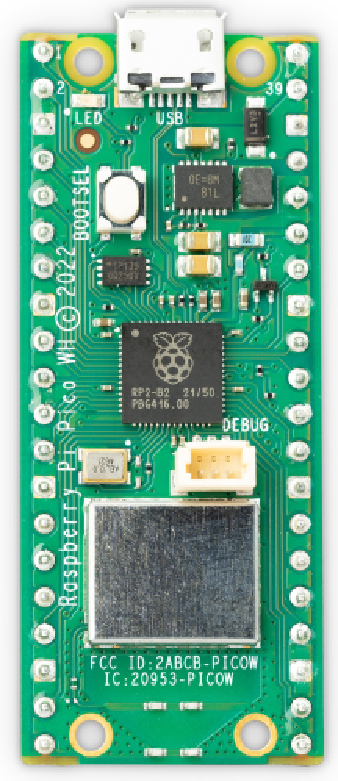
\includegraphics[width=.6\textwidth]{Imagenes/Vectorial/piPicoWH.pdf}
        \caption{Raspberry Pi Pico WH}
        \label{fig:piPicoWH}
    \end{minipage}
\end{figure}


%
% Single-board Computers
%
\subsection{Single-board Computers}

A single-board computer (\textit{SBC}) is a complete computer built on a single circuit board. It integrates all 
the necessary components required for a functional computer system, including a central processing unit (CPU), 
memory (RAM), storage (usually in the form of a MicroSD card), input/output ports, and sometimes additional 
features such as networking capabilities (e.g., Ethernet or WiFi), audio/video output, GPIO (General Purpose 
Input/Output) pins for connecting external devices, and even USB ports.

SBCs are designed to be compact and efficient, which is the case of the \textit{Pi Zero}, measuring about 65mm by 
30mm while drawing about one Watt of power. Additionally, SBCs can run an operating system, such as Ubuntu.

This ability to run an entire operating system significantly enhances their versatility compared to microcontrollers 
out-of-the-box. Many peripheral devices can simply be plugged into a USB port and function seamlessly without 
requiring additional configuration. For instance, a 3G SIM card adapter, which will be necessary for future stages 
of the project, can be effortlessly integrated into the system, letting the operating system take charge of the 
communication with the mobile network, abstracting all these problems from the programmer.


%
% Microcontrollers
%
\subsection{Microcontrollers}

A microcontroller is a compact integrated circuit (IC) that contains a central processing unit (CPU), memory (both 
volatile RAM and non-volatile flash memory), input/output peripherals (such as digital and analog I/O pins), and 
various other hardware components necessary for interfacing with external devices. Unlike single-board computers, 
microcontrollers are typically designed for specific tasks and embedded applications, often with real-time requirements.

One key characteristic of microcontrollers is their ability to execute dedicated firmware or software code stored in 
their internal memory. This code typically controls the behavior of the microcontroller, processes inputs from sensors 
or other external devices, and generates outputs to control actuators or display information.

The \textit{Raspberry Pi Pico W} is a development board that utilizes the \textit{RP2040} microcontroller chip. This board 
offers a range of features beyond its microcontroller, including onboard flash memory for program storage, versatile 
GPIO pins for interfacing with external devices, built-in USB connectivity for programming and power supply, and 
WiFi connectivity.

In comparison to single-board computers, the \textit{Pi Pico} does not have an operating system. Instead, firmware can be 
loaded onto it, and it is this firmware that provides functionality to the board. This firmware allows the programmer to 
use programming languages such as C or MicroPython, which then control the microcontroller's behavior and interactions with 
external devices.

The absence of an operating system reduces the overhead associated with system management and resource allocation, resulting 
in faster boot times and improved reliability for time-critical tasks.

Taking into account our previously established requirements, which prioritize minimal points of failure, low computational 
demands, and cost-effectiveness, the logical preference leans towards the utilization of a microcontroller. For instance, 
single-board computers often rely on SD cards for storage, which can be prone to failure after prolonged use due to factors 
such as wear and tear or data corruption. In contrast, microcontrollers typically have simpler storage mechanisms, such as 
onboard flash memory, which are less susceptible to such issues. Thus, lower operating costs.

As a conclusion, a \textbf{microcontroller will be used}, and in particular, the \textit{\textbf{Raspberry Pi Pico W}}.

%
% Electronic Modules
%
\subsection{Electronic Modules}

Now that the microcontroller has been selected, additional components are necessary to meet the project's requirements. 
Specifically, the device must integrate an NFC reader and an LCD screen. Additionally, other peripherals, such as a buzzer 
or LED, may also be evaluated.

We need to take into account the available buses and choose modules accordingly. Relying solely on the datasheet alone is 
not enough to determine the buses that are usable concurrently, since if two different buses use the same pin, then they 
cannot be used simultaneously. Referring to the pinout diagram of the \textit{Raspberry Pi Pico W} provided below, we can 
identify the available buses:

\begin{figure}[h]
	\centering
	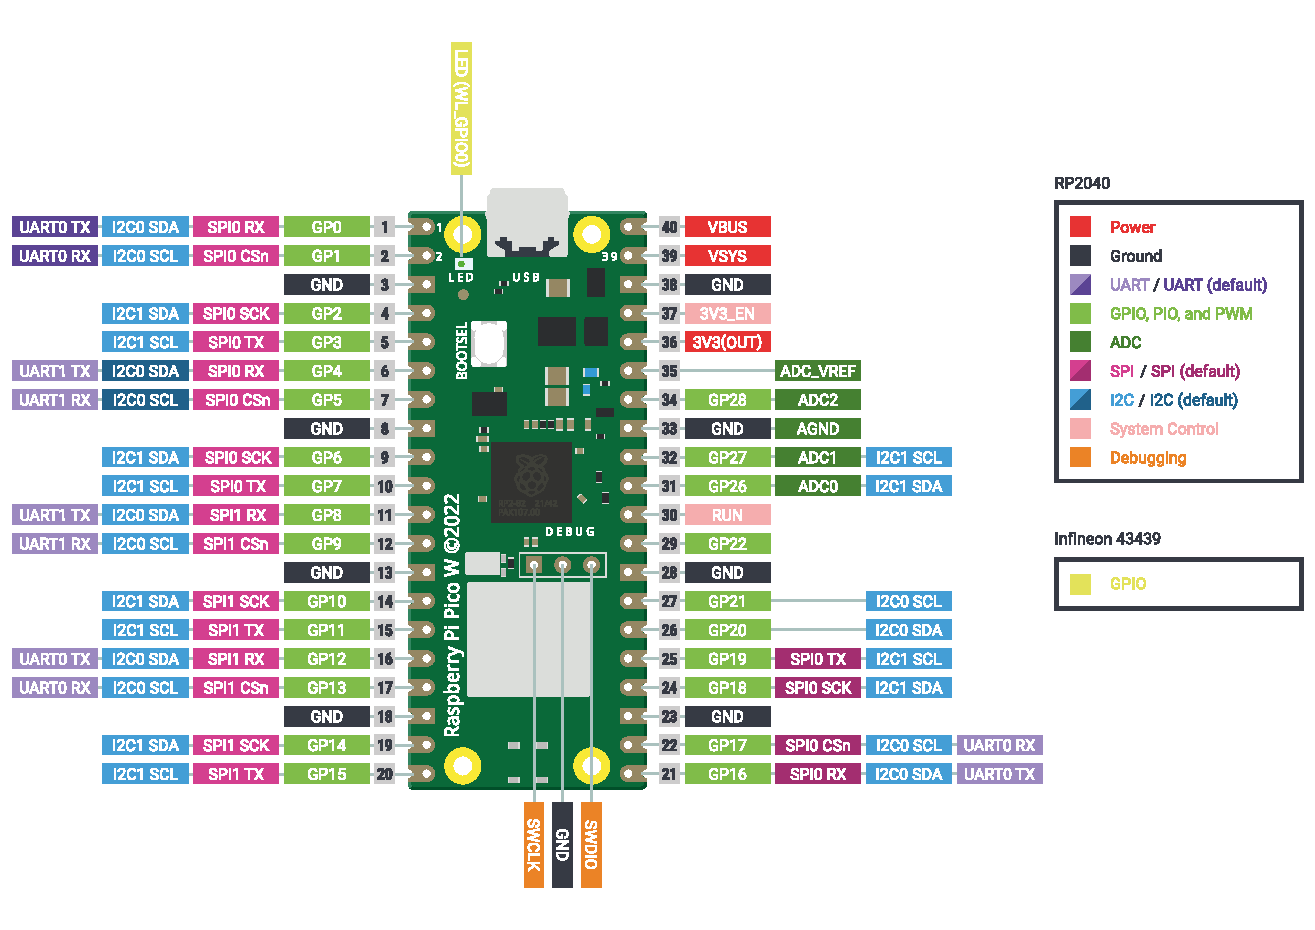
\includegraphics[width = 1\textwidth]{Imagenes/Vectorial/picow-pinout.pdf}
	\caption{Raspberry Pi Pico W's Pinout}
	\label{fig:piPicoPinout}
\end{figure}

For example, each UART bus conflicts with I2C buses. Therefore, when selecting components, it's crucial to ensure 
compatibility with this layout \cite{raspberrydocs}.


\subsubsection*{NFC Module}

Various NFC boards are available on the market. Ideally, the desired NFC board would offer extended range, compact 
form-factor, low power consumption, and support for multiple communication protocols such as UART, I2C, SPI, among others.

The \textit{PN532} chipset produced by \textit{NXP} offers all three types of buses mentioned before, that is: High Speed 
UART, I2C and SPI. Numerous boards utilizing this chipset are available on the market, with \textit{ElecHouse}'s offering 
standing out for its excellent form-factor (about 4cm$\times$4cm) and impressive range \cite{pn532_elechouse}. This specific board has been 
extensively replicated and is accessible at a low cost, and various providers offer open-source code for controlling it.

\begin{figure}[h]
	\centering
	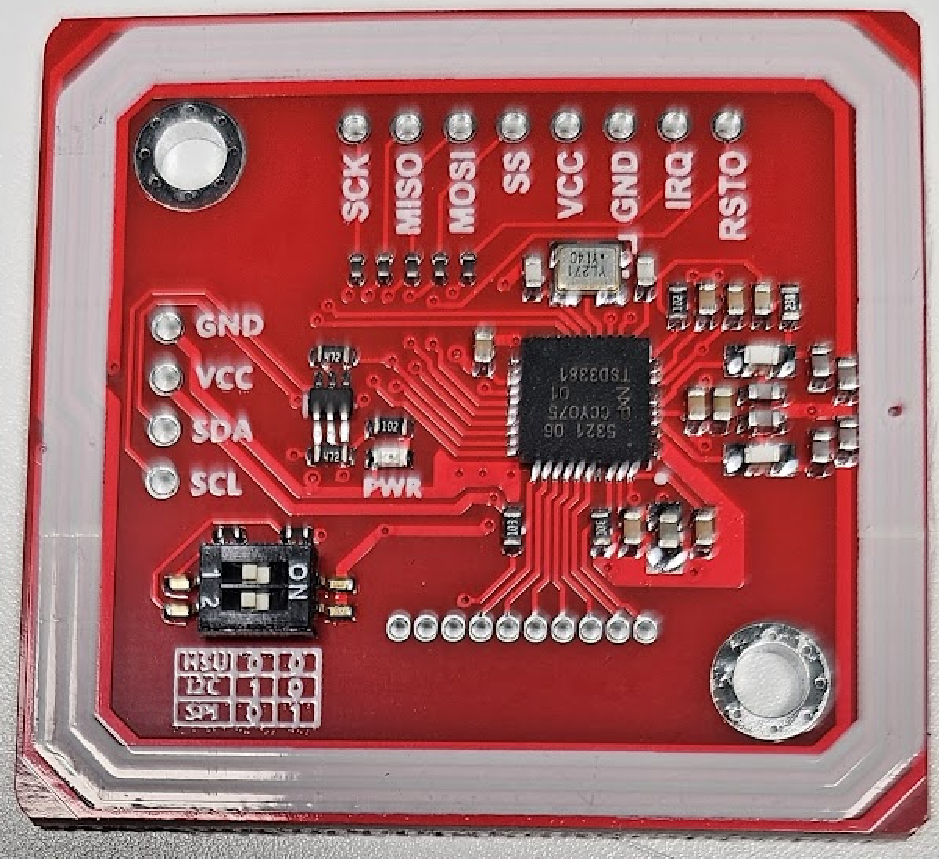
\includegraphics[width = 0.3\textwidth]{Imagenes/Vectorial/PN532.pdf}
	\caption{PN532 board}
	\label{fig:pn532}
\end{figure}

\subsubsection*{LCD Module}

Initially, the idea of utilizing a black and white OLED display seemed appealing. However, as the size increased, so did 
the price, and even then, the displays were still too small. Consequently, the most practical decision was to adhere to 
LCD technology.

Upon researching LCD modules, the \textit{LCD1602} module emerged as a suitable choice. It offers sufficient size, 
accommodating up to 16 characters per row across 2 rows, and provides satisfactory contrast. Additionally, it is 
available with I2C adapters for simplified control, requiring fewer pins on the microcontroller.

\begin{figure}[h]
	\centering
	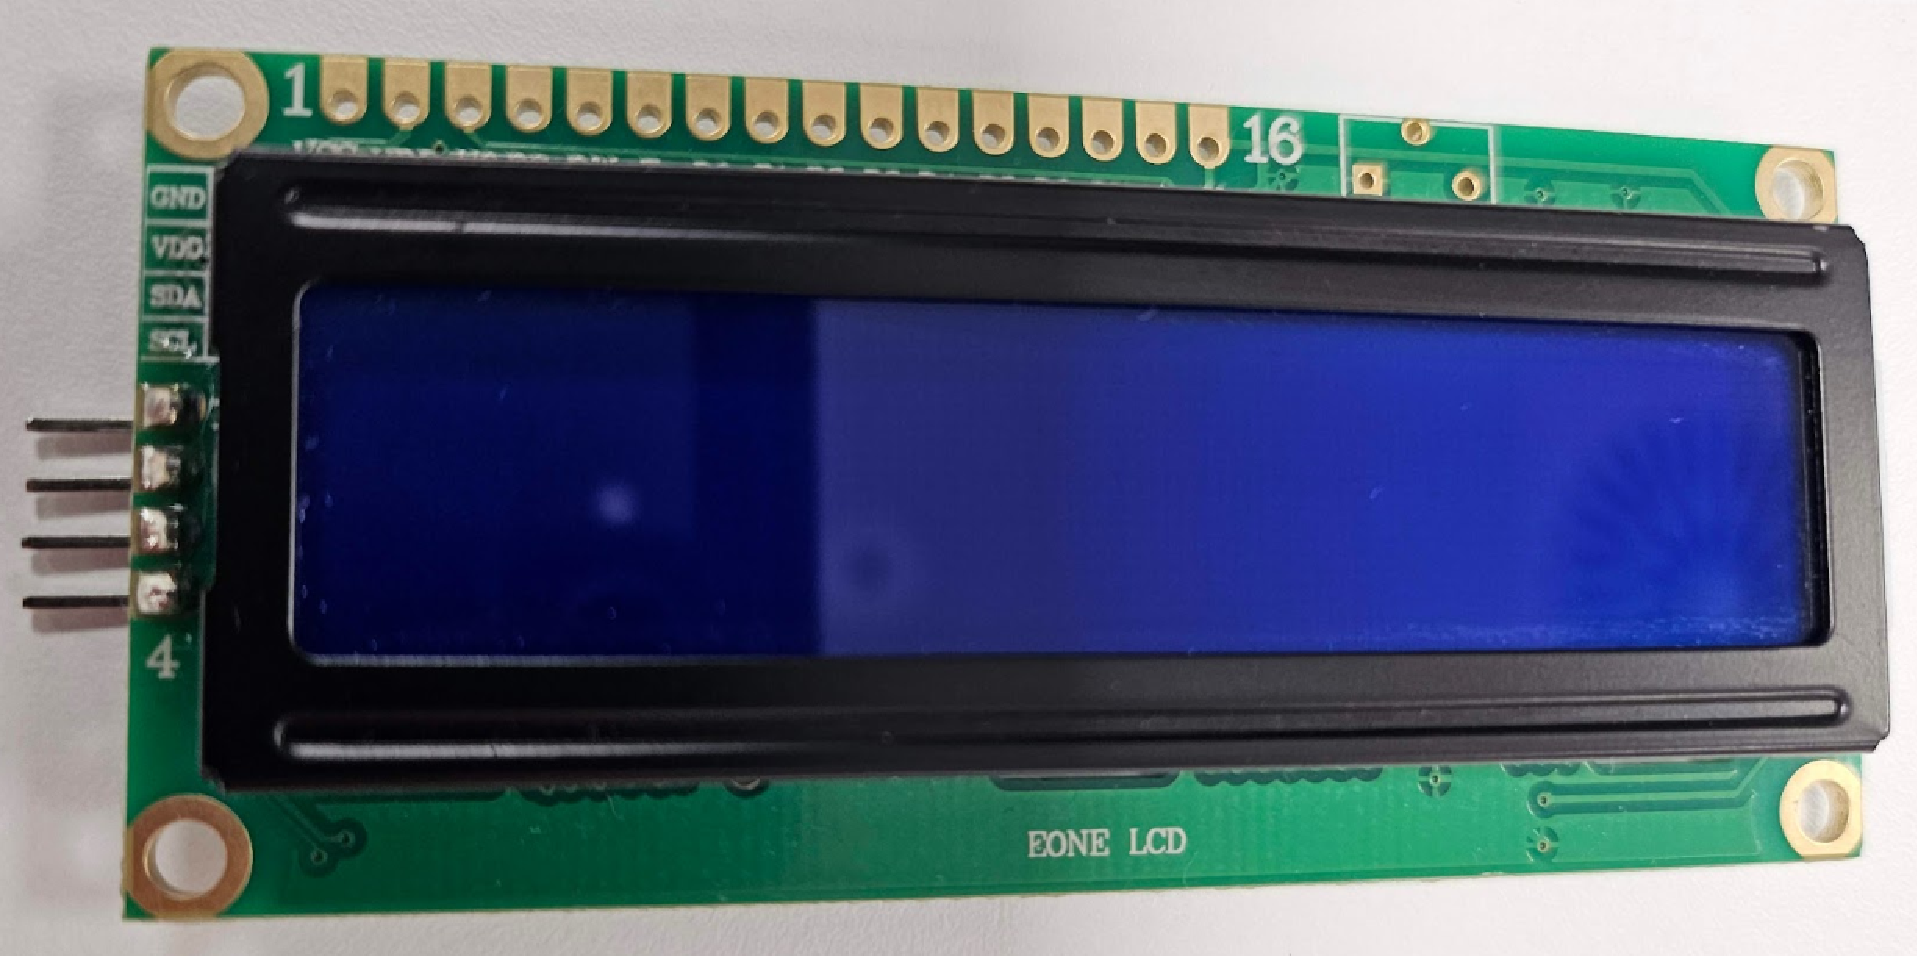
\includegraphics[width = 0.7\textwidth]{Imagenes/Vectorial/LCD1602.pdf}
	\caption{LCD1602 board}
	\label{fig:lcd1602}
\end{figure}


\subsubsection*{Buzzer}

Beyond just relying on visual cues displayed on the screen to convey the device's status, it's essential to enhance 
the user experience by incorporating auditory feedback. When employees clock in to work, providing a distinct sound 
signal from a buzzer ensures they receive immediate confirmation of their action.

There are two types of buzzer:
\begin{itemize}
	\item \textbf{Active buzzers}: they incorporate an internal oscillator circuit that generates the sound signal 
	when voltage is applied. They are self-contained and do not require external circuitry to produce sound. They 
	are commonly used in applications where simplicity and ease of use are prioritized, as they can be directly 
	connected to a power source to emit sound.
	\item \textbf{Passive buzzers}: they require an external oscillating circuit to produce sound. An alternating 
	current is applied to create vibrations that produce sound waves. They offer more flexibility in sound frequency 
	and intensity control but require additional circuitry for operation.
\end{itemize}

Due to the project's time constraints and the preference for simplicity, \textbf{active buzzers will be employed}. 
Additionally, since a single sound frequency suffices for the intended use, active buzzers are well-suited for the task.


\subsubsection*{Cellular Connectivity Module}

In certain locations, access to WiFi networks may be limited or unavailable altogether. Even in areas where WiFi is 
accessible, signal strength may vary, leading to instances of poor connectivity. Consequently, it becomes imperative 
to incorporate cellular connectivity options to ensure internet access across diverse environments and conditions. By 
integrating cellular connectivity capabilities into the system, users can rely on alternative means of internet access, 
mitigating the limitations posed by WiFi availability and signal quality fluctuations.

Considering the time limitations, it would be benefitial to opt for a ready-made solution. However, it's worth noting 
that the Raspberry Pi Pico, being a microcontroller, cannot simply utilize a USB dongle with a SIM card adapter for 
cellular connectivity. A more intricate solution is necessary. Fortunately, there exists a module specifically designed 
for compatibility with the Pi Pico, developed by \textit{Waveshare}. This module integrates the \textit{SIM7020E} module, 
manufactured by \textit{SIMCOM}, a prominent provider of wireless modules and electronics.

The \textit{SIM7020E} module, known for its affordability and low power consumption, is specifically designed for 
NB-IoT\footnote{NB-IoT, short for Narrowband Internet of Things, is a low-power cellular technology designed for efficient 
communication between IoT devices and networks.} applications, making it an optimal choice for M2M\footnote{M2M stands 
for Machine-to-Machine, and encompasses a wide range of applications where devices or machines communicate and exchange 
data without human intervention.} communication scenarios. Integrated into the \textit{Waveshare} board, this module 
establishes communication with the Pi Pico through UART, using \textit{AT}\footnote{AT commands are a standardized set of 
instructions used to communicate with and control modems and other serial devices.} commands for control and data exchange 
\cite{sim7020e_datasheet}.

However, a significant tradeoff exists as this module only supports NarrowBand IoT. NB-IoT operates within the LTE 
(Long-Term Evolution) spectrum and is tailored for narrow bandwidths, making it ideal for low-power, wide-area IoT 
applications. While NB-IoT typically utilizes the 4G LTE spectrum, it operates at reduced data rates compared to 
conventional LTE, facilitating efficient communication with IoT devices while minimizing power consumption and costs.

Nonetheless, this limitation poses challenges as the range constraints of LTE networks persist, potentially leading to 
signal issues in underground facilities. In an ideal scenario, a module supporting 2G and NB-IoT would be preferable for 
the project. However, such modules are not readily available on the market for seamless integration with the Pi Pico. While 
\textit{SIMCOM} does offer several variants of these modules with diverse capabilities, developing a custom solution would 
necessitate significant investment in terms of both time and resources.

However, the downside of this approach is that the module requires soldering of fourteen pins (the ones whose text is highlighted in white in Fig. \ref{fig:sim7020e_bottomview}), introducing an additional layer of complexity to the device assembly process. Furthermore, it is important to note the stacking headers featured in Figures \ref{fig:sim7020e_topview} and \ref{fig:sim7020e_bottomview}, which consist of female headers with extended male pins. These pins are designed to penetrate the PCB and connect to another female header underneath. While this setup may appear standard, improper soldering, with excess tin reaching too high on the male part of the header, can lead to faulty connections with the PCB or breadboard. Therefore, if the team intends to assemble the device on-site, careful soldering is a must.

\begin{figure}[h]
    \centering
    \begin{minipage}[b]{0.45\textwidth}
        \centering
        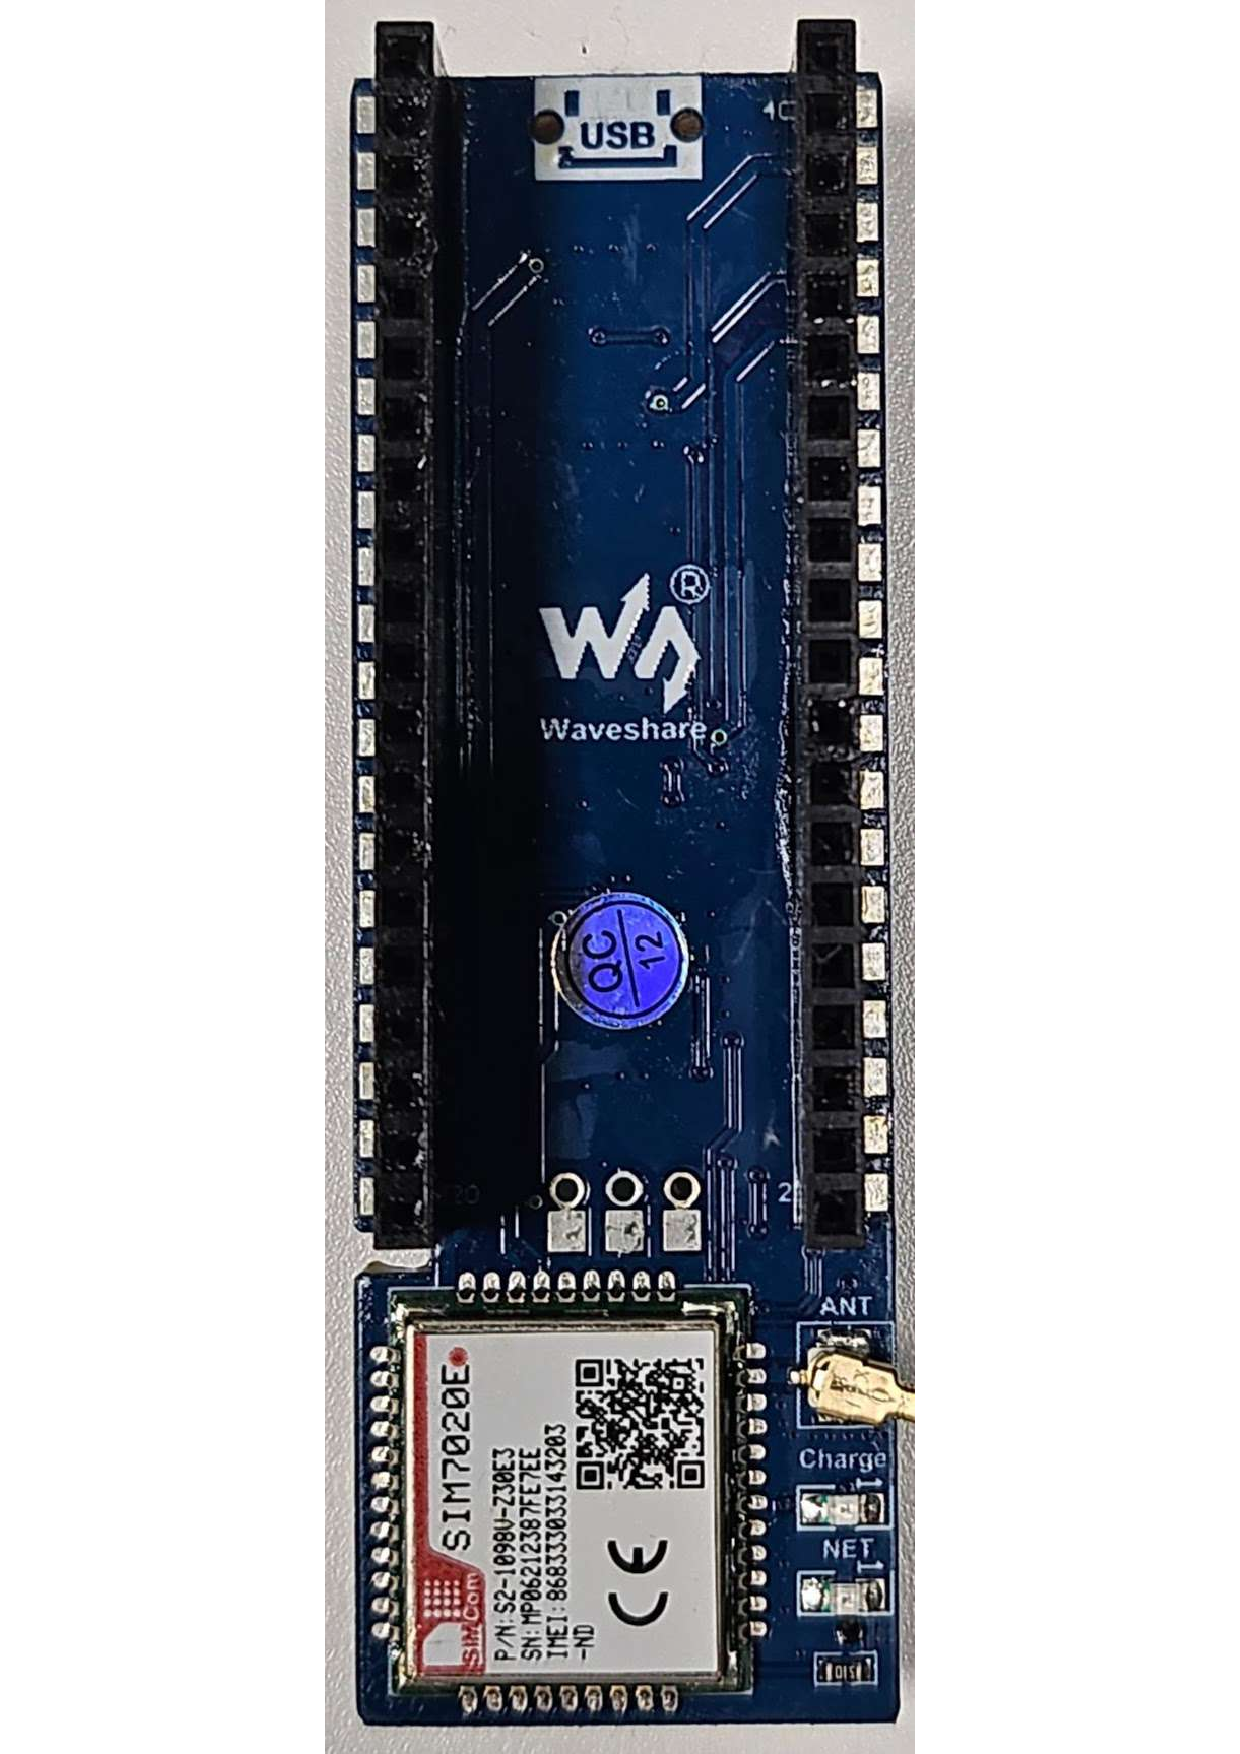
\includegraphics[width=.6\textwidth]{Imagenes/Vectorial/sim7020e_topside.pdf}
        \caption{Waveshare's SIM7020E module, top view}
        \label{fig:sim7020e_topview}
    \end{minipage}
    \hfill
    \begin{minipage}[b]{0.45\textwidth}
        \centering
        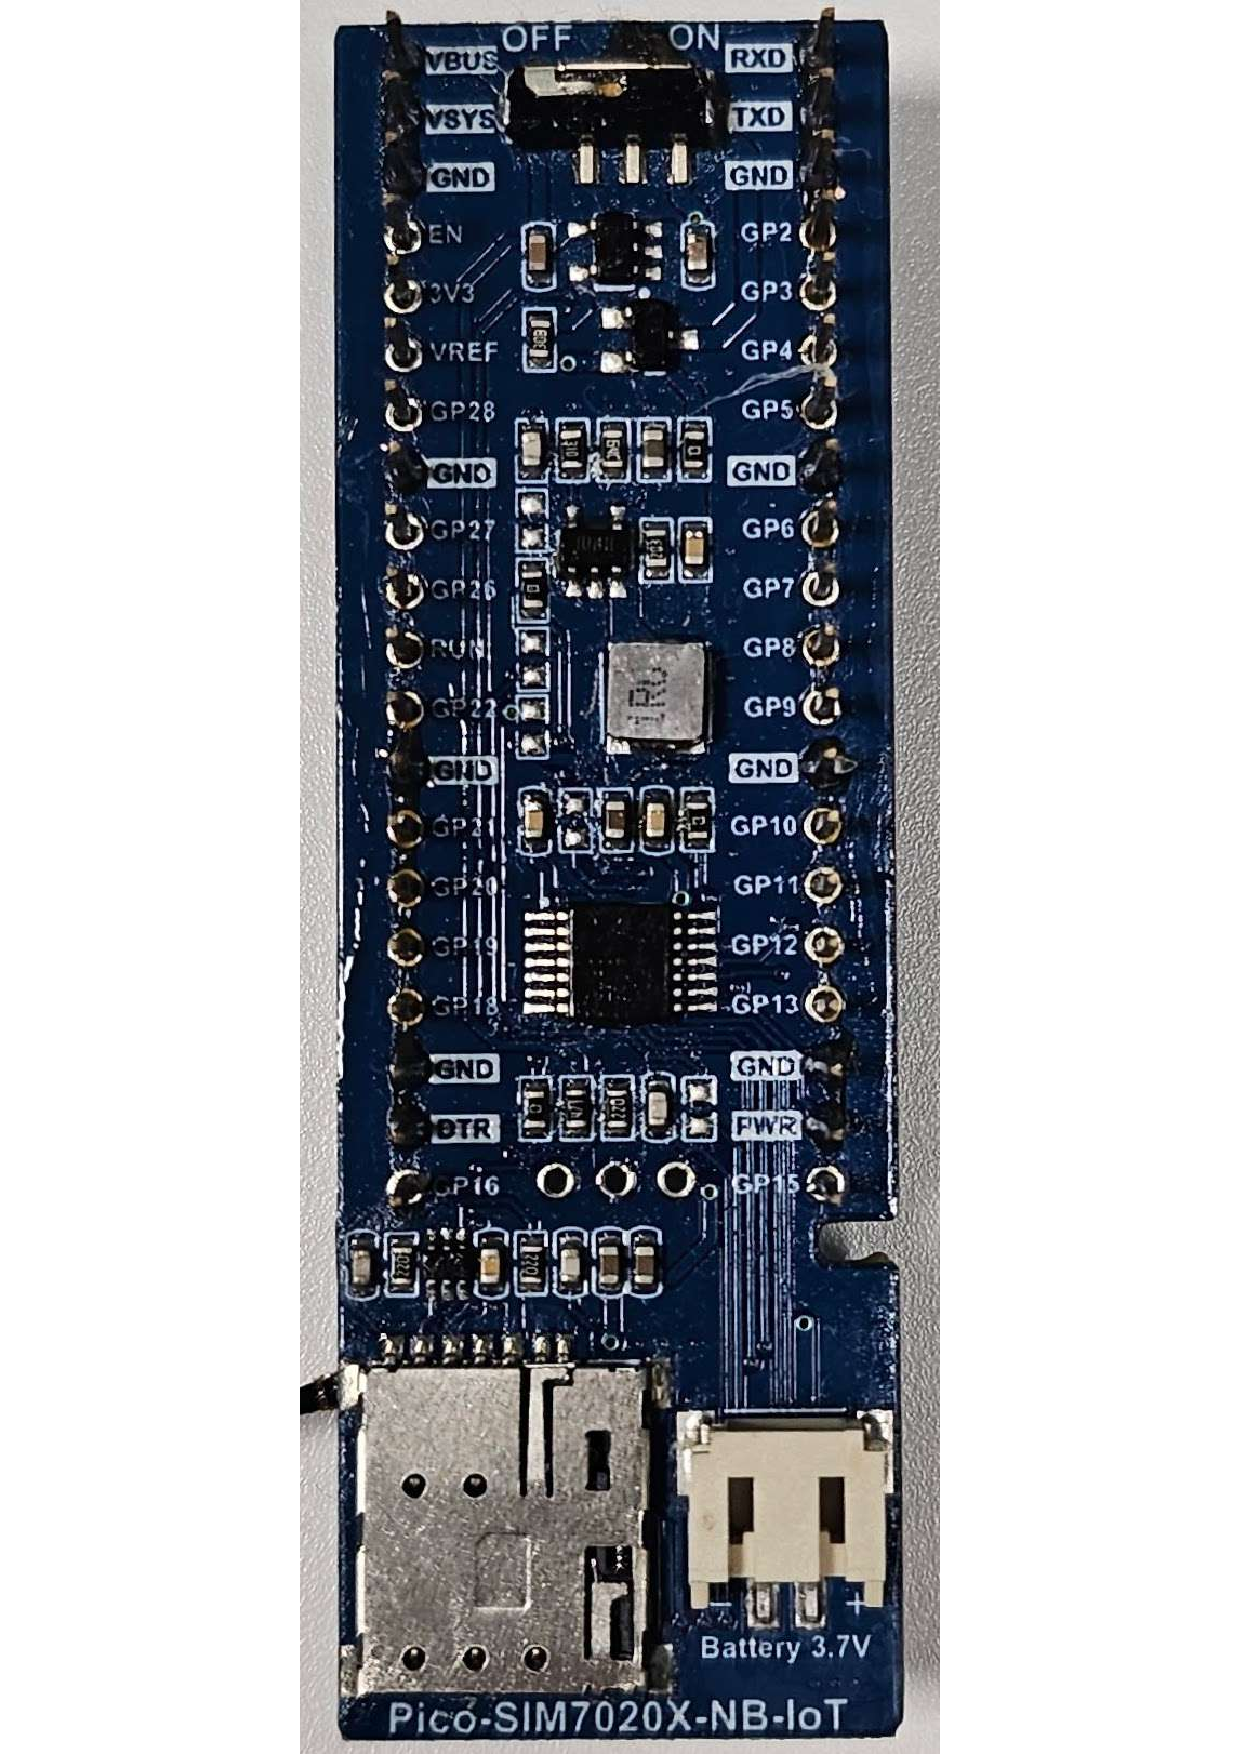
\includegraphics[width=.6\textwidth]{Imagenes/Vectorial/sim7020e_bottomside.pdf}
        \caption{Waveshare's SIM7020E module, bottom view}
        \label{fig:sim7020e_bottomview}
    \end{minipage}
\end{figure}


\subsubsection*{Buses}

As previously mentioned, various buses are available for interconnecting components. While the LCD is already set up 
for I2C, the NFC reader offers more flexibility in bus selection. However, to maintain simplicity, the NFC reader will 
also utilize the I2C bus.

I2C, short for Inter-Integrated Circuit, is a serial communication protocol commonly utilized for connecting 
microcontrollers and peripheral devices. It operates using two wires: \textit{SDA} (Serial Data) and \textit{SCL} (Serial 
Clock). Devices connected to the bus are addressed individually by unique addresses, and communication follows a 
master-slave configuration. The master device initiates communication and controls the bus, while one or more slave devices 
respond to commands. Data is transferred sequentially, with the master device generating clock pulses to synchronize 
communication \cite{nxpi2c}.

However, I2C does have limitations. It operates at relatively low speeds compared to other protocols, which can impact 
performance in applications requiring high data transfer rates. The length of the I2C bus is also limited due to signal 
integrity issues, typically to a few meters, which may restrict the physical layout of devices in larger systems. In any 
case, none of these limitations affect this project's use case.

The \textit{Pi Pico} features two I2C buses, providing an additional bus beyond what is required. It's important to mention 
that the two modules can share the same I2C bus since they have different I2C addresses. For instance, the PN532 always uses 
the \textit{0}x\textit{48} address, which cannot be modified. Consequently, two PN532 readers cannot share the same bus and 
must be placed separately. However, this is not an issue for the LCD as it uses a different address.

Note: While the PN532 produced by \textit{NXP} does allow for the modification of the I2C address \cite{nxp_pn532}, it is 
conventionally maintained at \textit{0}x\textit{48} \cite{i2cdevices_pn532}.


\subsubsection*{Matrix Keypad}

A matrix keyboard offers an alternative means for employees to clock in or out by entering a numeric code, which can be 
particularly useful if an employee forgets or misplaces their card. The working principle of matrix keyboards is 
straightforward: as illustrated in Figure \ref{fig:matrix_keypad_schematics}, they consist of intersecting rows and columns. 
Each key on the keyboard is positioned at the intersection of a row and a column. When a key is pressed, it creates a 
connection between a specific row and column, resulting in a unique electrical signal that can be interpreted by the 
microcontroller.

\begin{figure}[h]
    \centering
    \begin{minipage}[b]{0.45\textwidth}
        \centering
        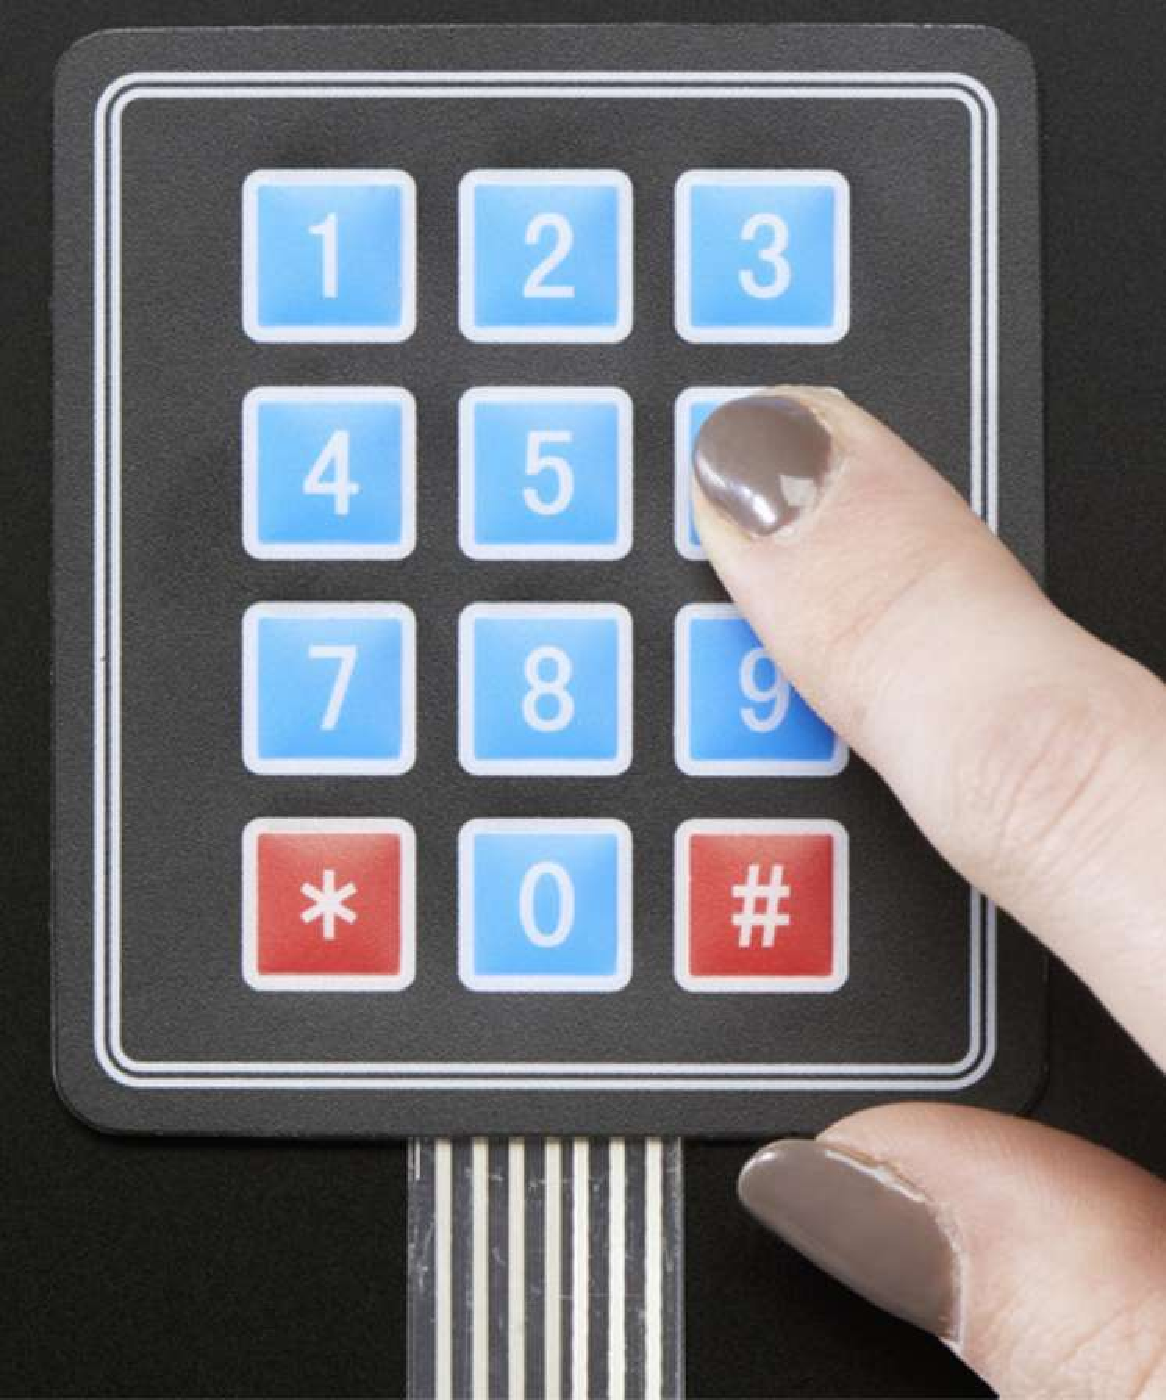
\includegraphics[width=.8\textwidth]{Imagenes/Vectorial/matrix_keypad.pdf}
        \caption{Matrix keypad}
        \label{fig:matrix_keypad}
    \end{minipage}
    \hfill
    \begin{minipage}[b]{0.45\textwidth}
        \centering
        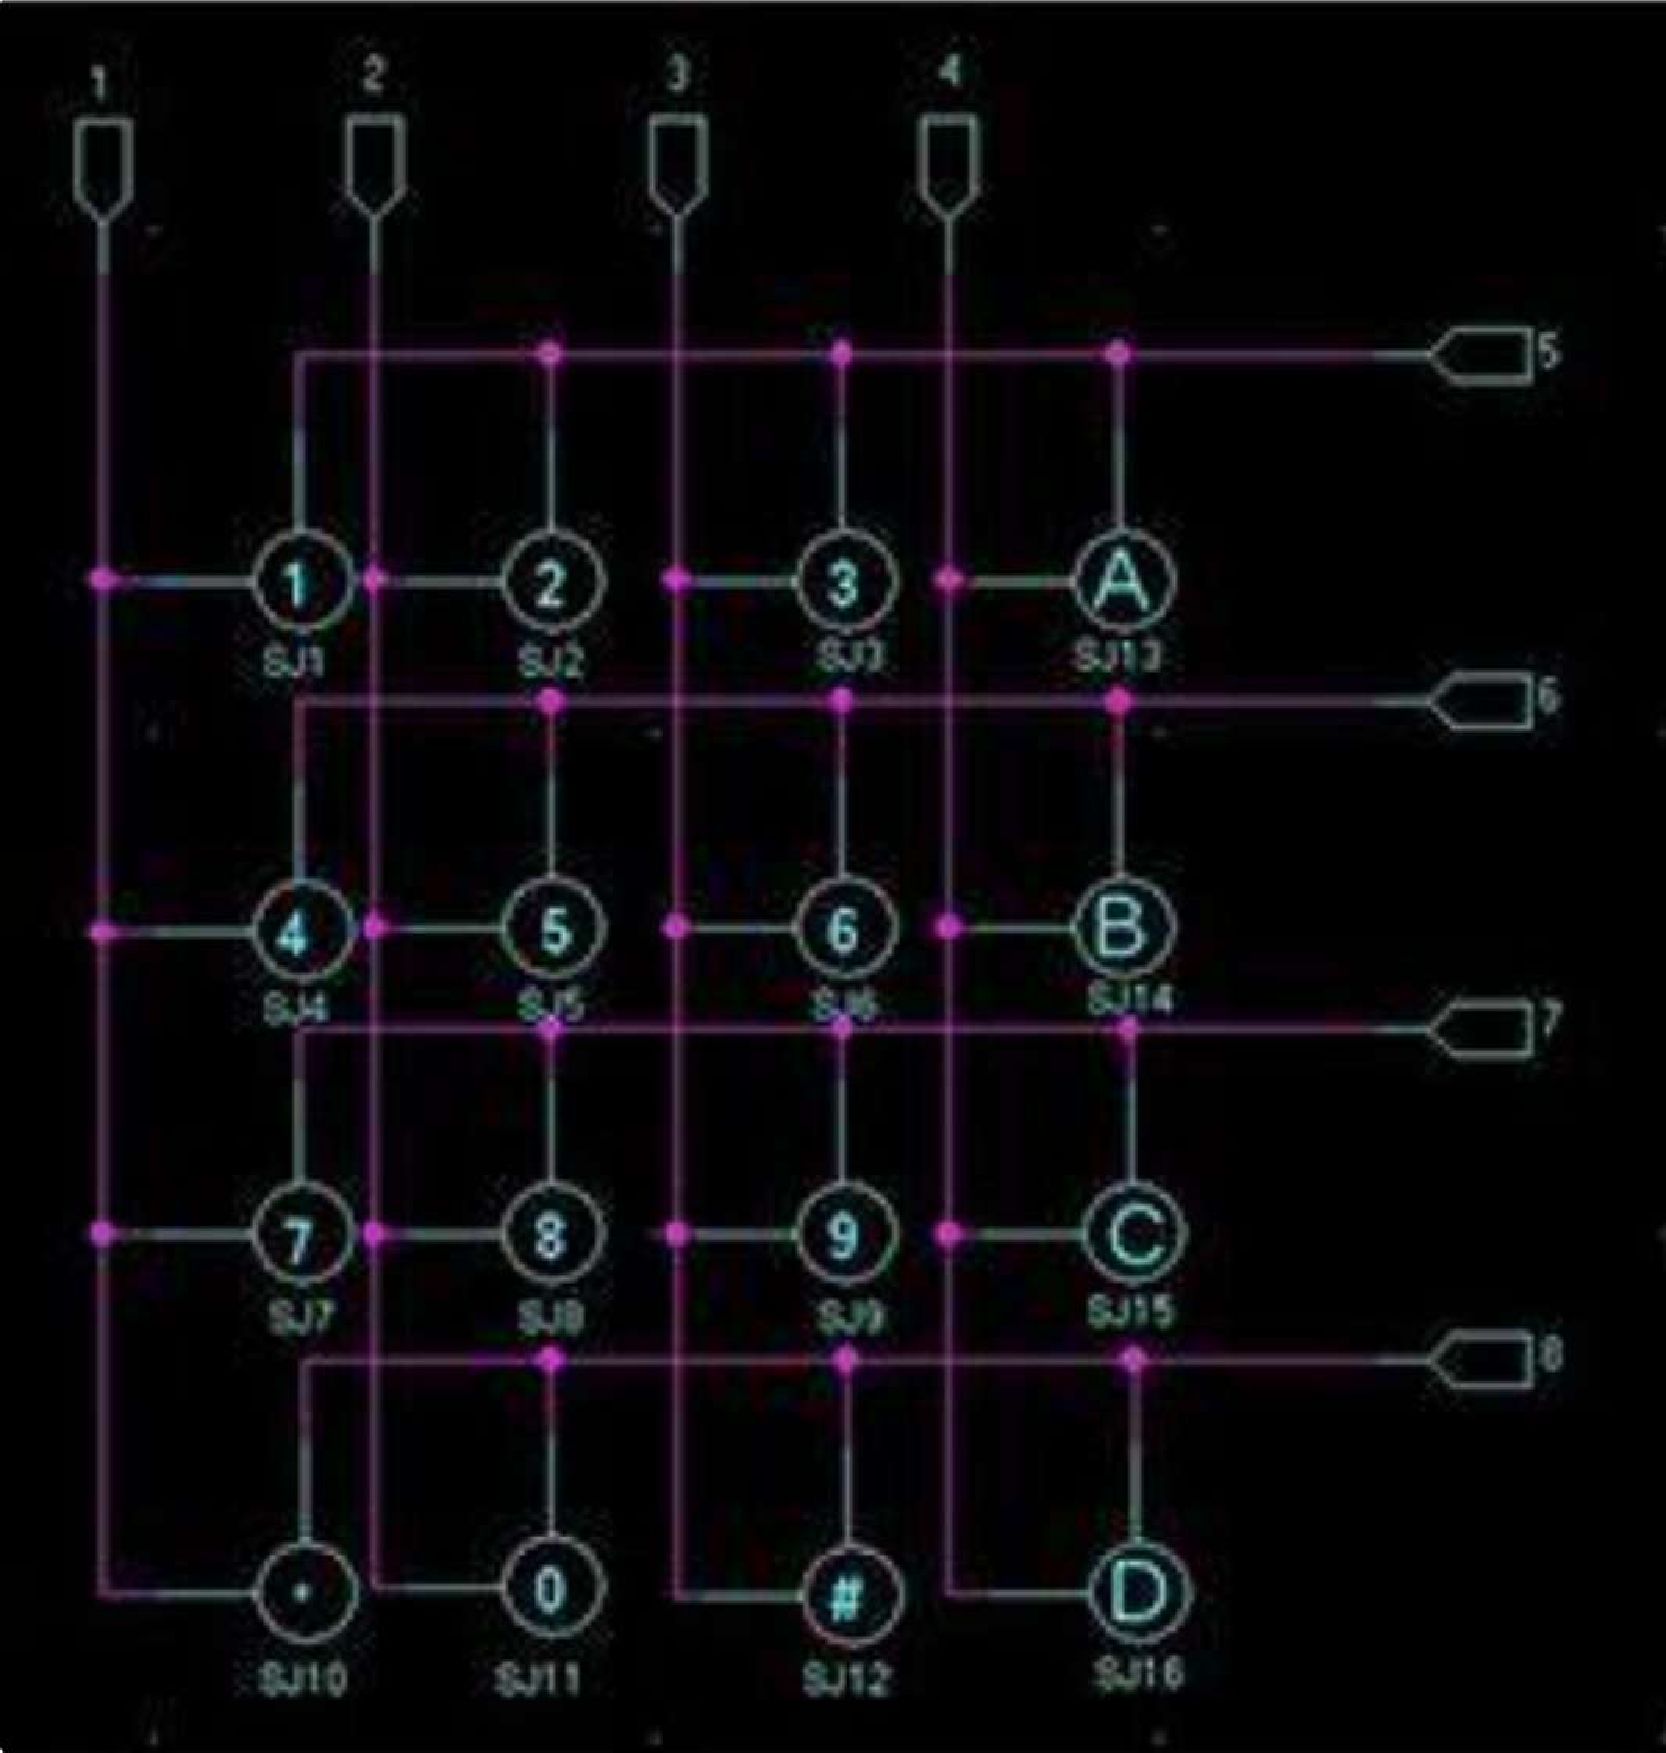
\includegraphics[width=.8\textwidth]{Imagenes/Vectorial/matrix_keypad_schematics.pdf}
        \caption{Matrix keypad's schematics}
        \label{fig:matrix_keypad_schematics}
    \end{minipage}
\end{figure}


Matrix keyboards utilize a scanning technique to detect key presses. The microcontroller sequentially activates each row, 
while monitoring the columns for any signals. If a signal is detected, the microcontroller identifies the corresponding key 
based on the activated row and column, allowing it to register the key press.

One important consideration when using matrix keyboards is the potential for key ghosting or masking. Ghosting occurs when 
multiple keys are pressed simultaneously, causing the keyboard to register unintended key presses. Masking, on the other hand, 
happens when certain key combinations prevent other keys from registering. To mitigate these issues, careful design and 
debounce techniques must be employed to ensure reliable key detection.

During testing, it was observed that with sufficiently fast scanning and debouncing, the occurrence of ghosting or masking on 
the keyboard would likely not present a problem in practical usage scenarios. This assessment stems from the understanding that 
the likelihood of multiple key presses happening simultaneously on a wall-mounted device, such as the one being developed, is 
minimal.

Another challenge arises from the substantial use of GPIO pins on the microcontroller. The 4$\times$4 keyboard depicted in 
Figure \ref{fig:matrix_keypad}, consisting of 4 rows and 4 columns, requires 8 GPIO pins for operation. Considering that the 
Pi Pico offers a total of 29 GPIO pins, this allocation accounts for nearly 30 percent of available pins.


%
%	Prototype Assembly
%

\section{Prototype Assembly}

Once the components have been selected and basic schematics drawn, the assembly process can commence. All components can be 
interconnected on a breadboard using jumper wires. It is important to highlight that the Raspberry Pi Pico WH comes with 
pre-soldered headers, facilitating easy integration for testing purposes. Only minimal soldering is required for certain 
components, such as the four pins on the NFC module and the fourteen pins for the Waveshare module.

Many of the components necessary for this prototyping phase can be obtained by purchasing a basic electronics kit, which 
typically includes a breadboard and jumper wires, and other basic components such as a matrix keyboard and buzzer.

In addition to the minor soldering required, the majority of components were effortlessly connected to the breadboard 
using jumper wires. The small footprint of the Pi Pico further simplified the connections to its pins.

\begin{figure}[h]
    \centering
    \begin{minipage}[b]{0.45\textwidth}
        \centering
        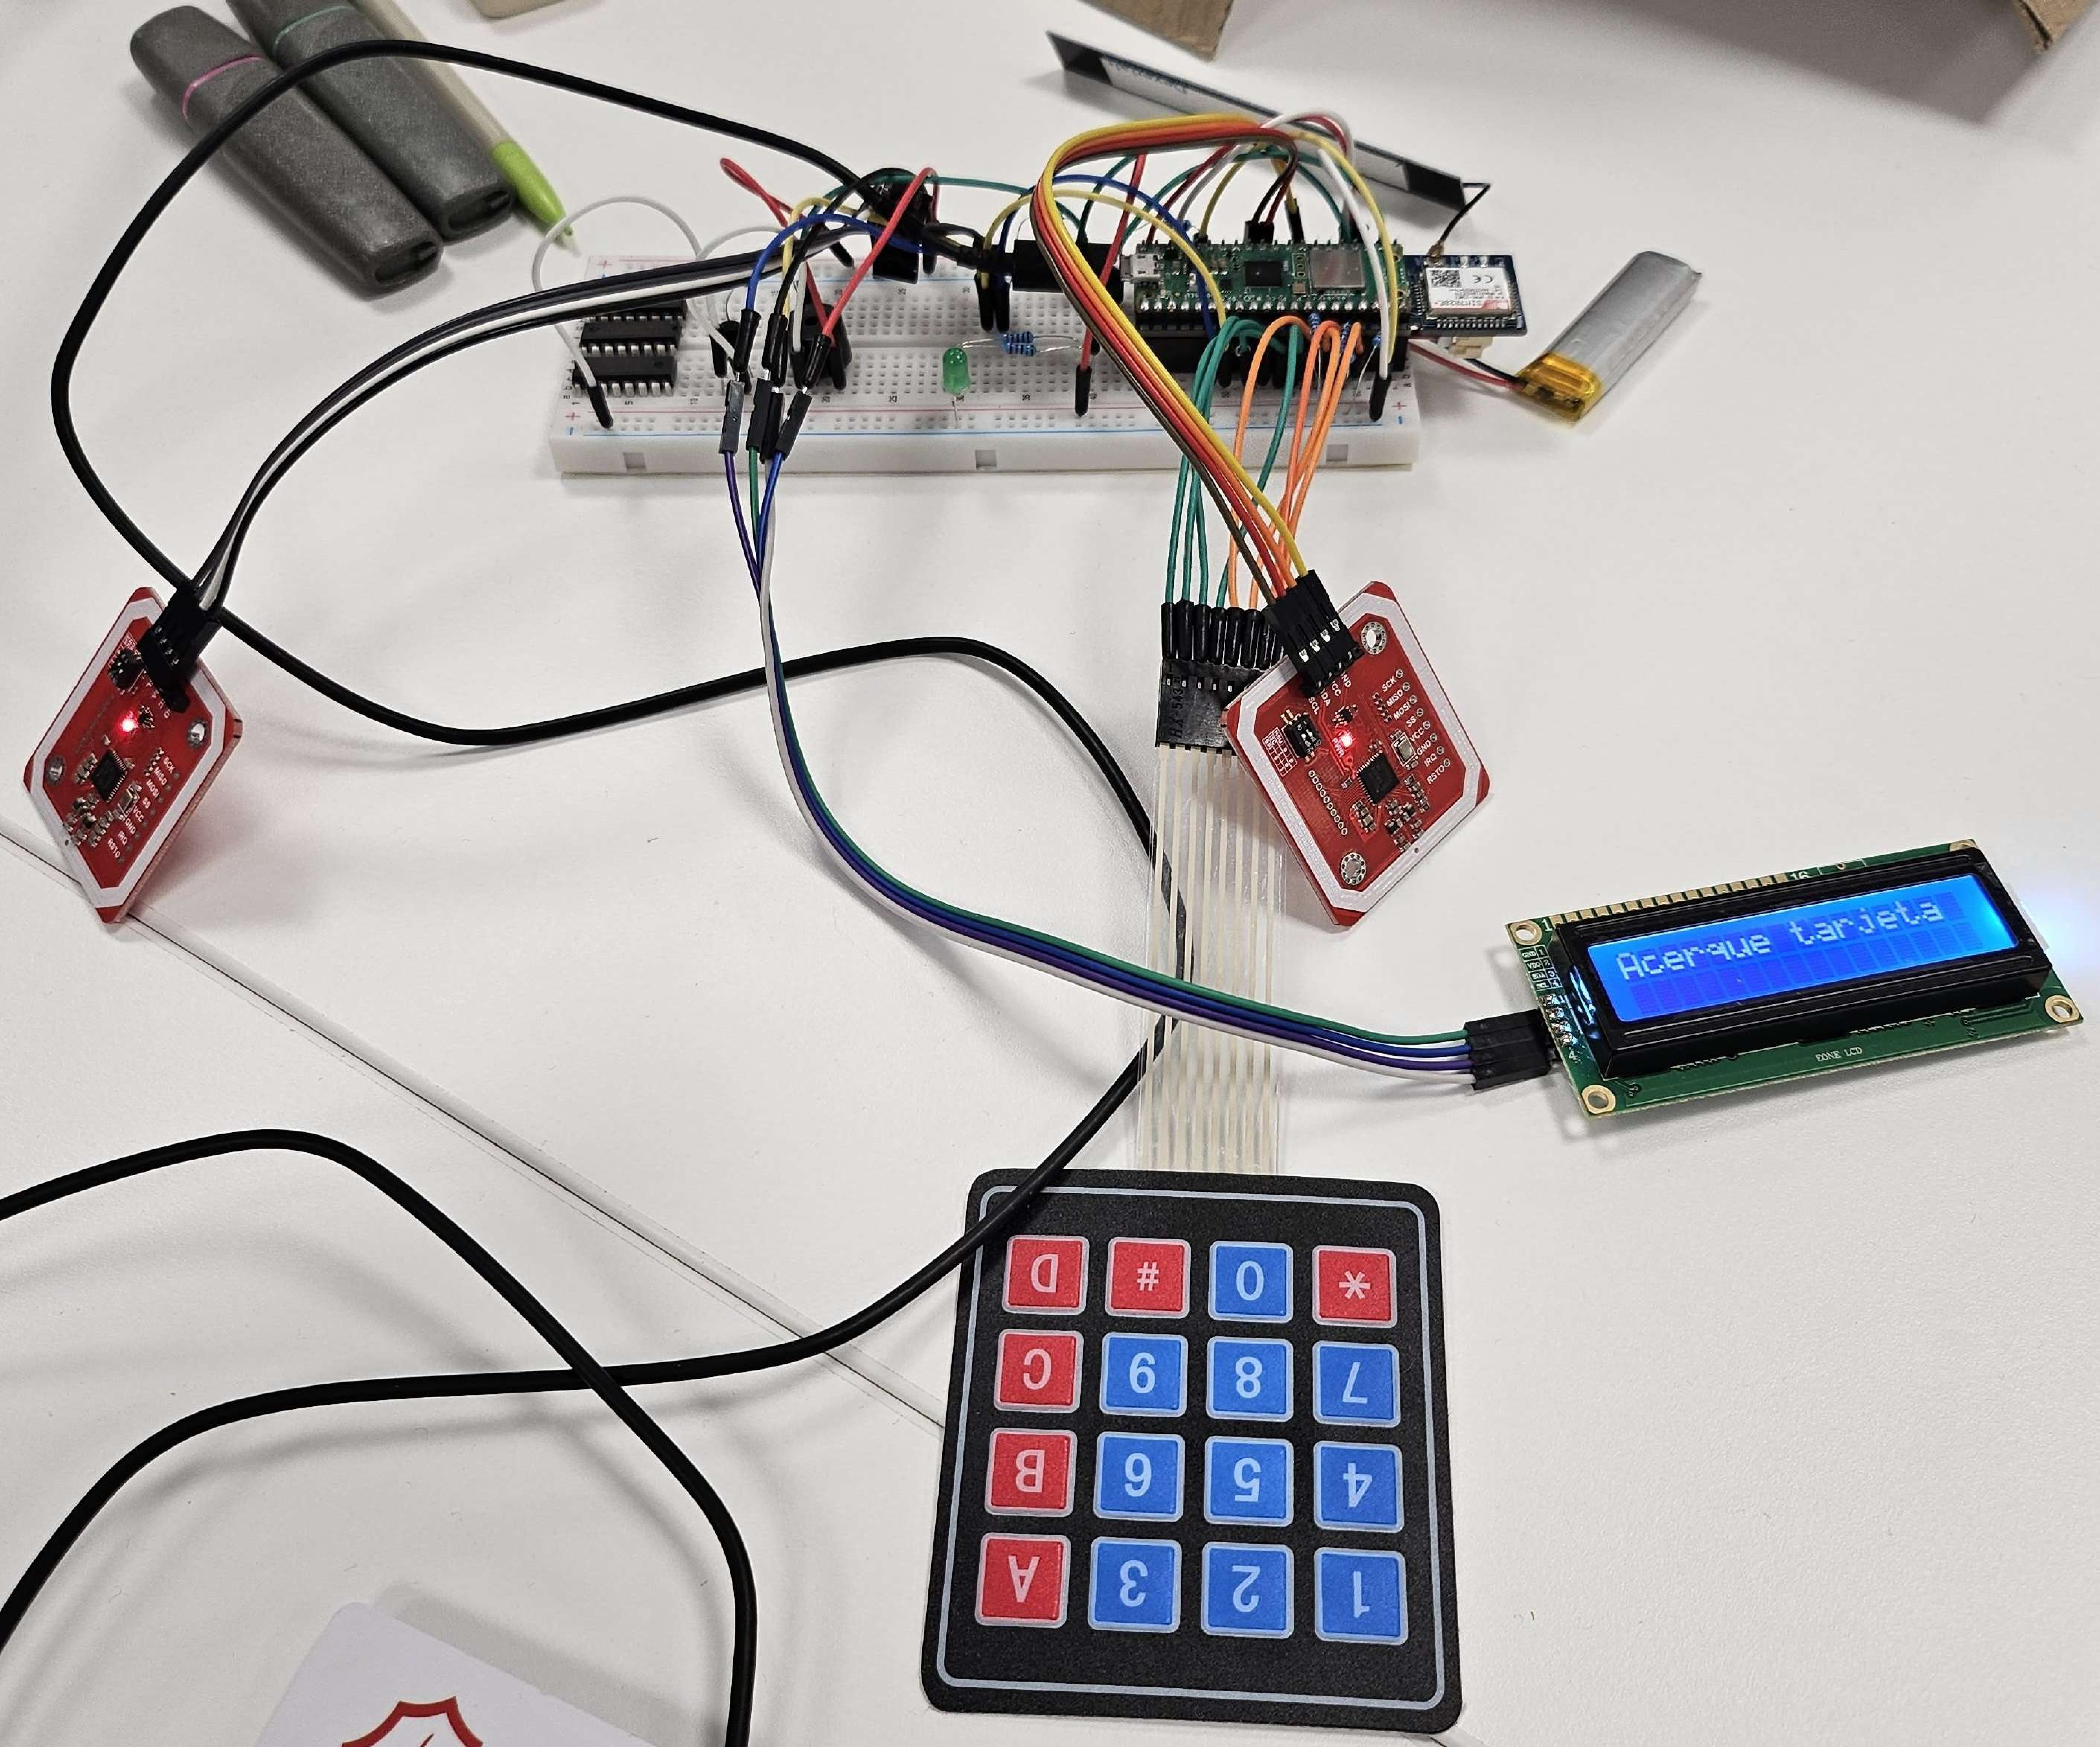
\includegraphics[width=1\textwidth]{Imagenes/Vectorial/breadboard1.pdf}
        \caption{First prototype mounted on a breadboard}
        \label{fig:breadboard1}
    \end{minipage}
    \hfill
    \begin{minipage}[b]{0.45\textwidth}
        \centering
        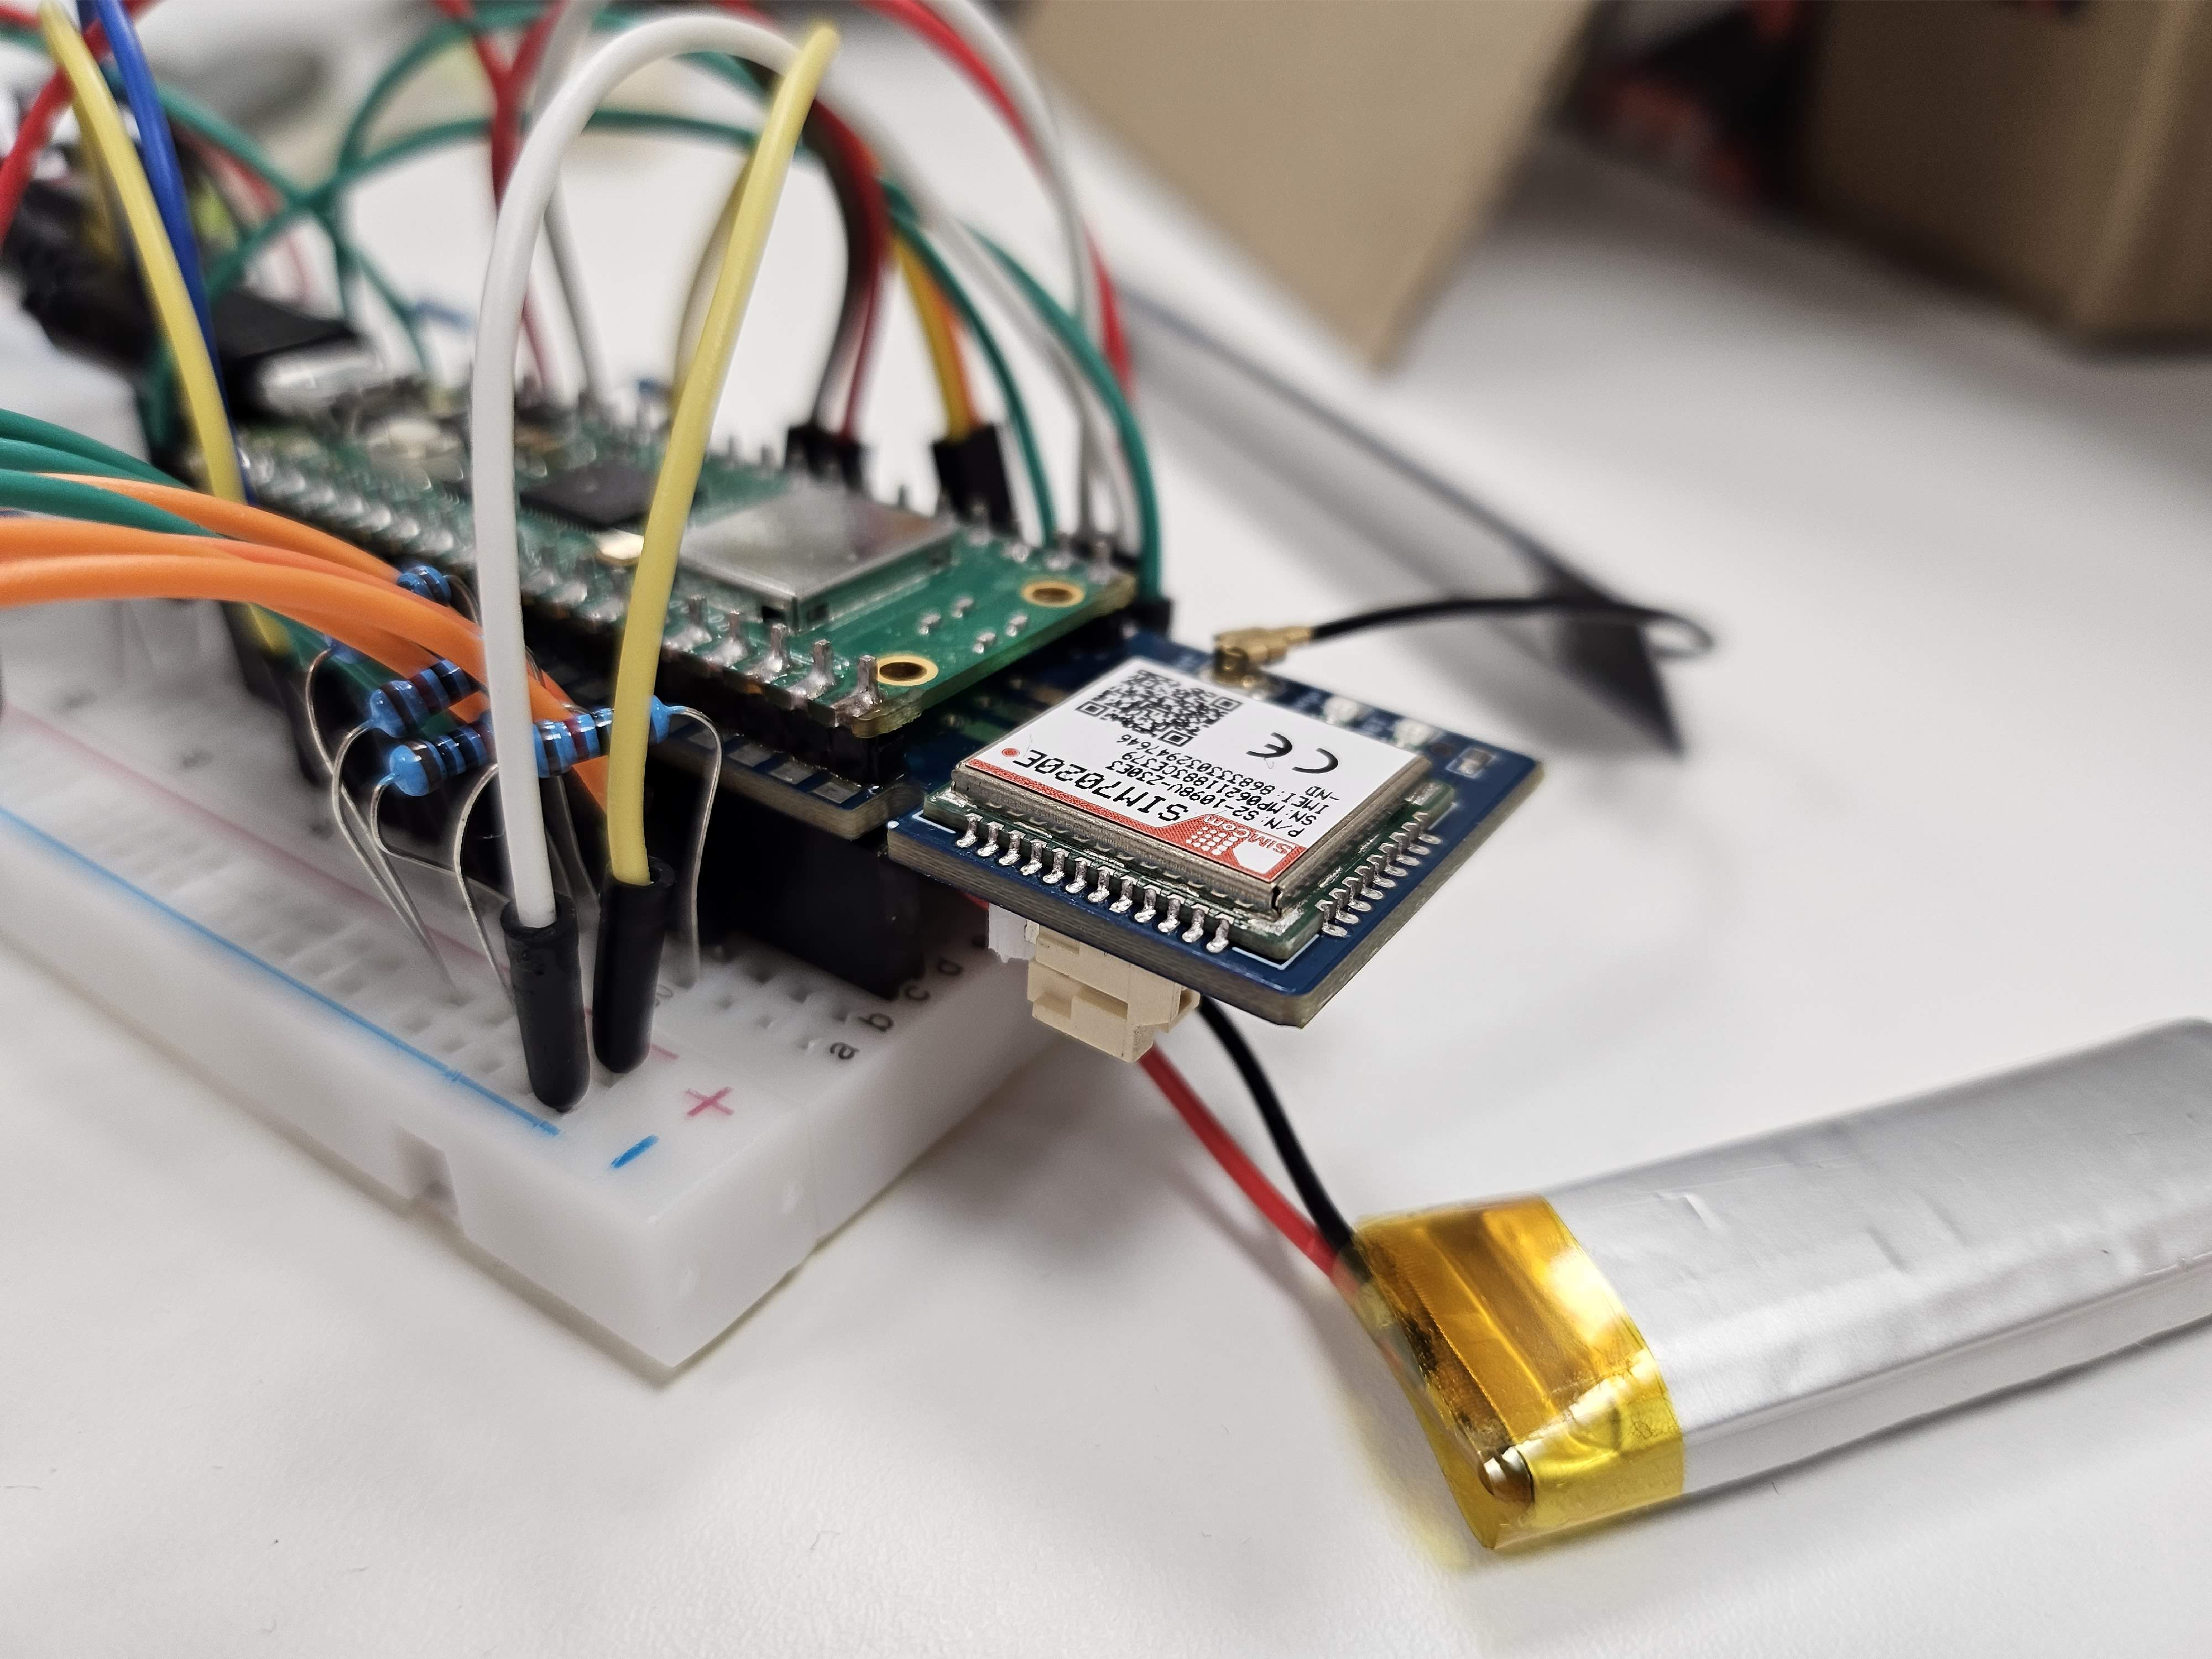
\includegraphics[width=1\textwidth]{Imagenes/Vectorial/breadboard2.pdf}
        \caption{Zoom in on the Pi Pico and SIM7020E module}
        \label{fig:breadboard2}
    \end{minipage}
\end{figure}

\subsubsection*{Considerations}

The initial prototype incorporated two NFC modules, as can be seen on figure \ref{fig:breadboard1}, intending to use one 
module for clocking in and the other for clocking out. This approach was adopted initially to streamline compatibility 
with a specific provider. However, this strategy was subsequently abandoned in favor of a simpler solution, whereby the 
worker's entry or exit status is determined through software processing.

Initially, the matrix keyboard was contemplated as an alternative method for clocking in or out by entering a numeric 
code. However, this approach was deemed impractical due to several concerns. Using the worker's national identification 
number as the input code would involve handling sensitive information, which was not ideal. Additionally, distributing 
individual codes to each worker would present logistical challenges. As a result, this approach was ultimately abandoned.


% \begin{figure}[h]
% 	\centering
% 	
\includegraphics[width = 0.5\textwidth]{Imagenes/Vectorial/Todo.pdf}
% 	\caption{Ejemplo de imagen}
% 	\label{fig:sampleImage}
% \end{figure}

% Si te sirve de utilidad,  puedes incluir tablas para mostrar resultados, tal como se ve en la tabla \ref{tab:sampleTable}.


% \begin{table}
% 	\centering
% 	\begin{tabular}{c|c|c}
% 		\textbf{Col 1} & \textbf{Col 2} & \textbf{Col 3} \\
% 		\hline\hline
% 		3 & 3.01 & 3.50\\
% 		6 & 2.12 & 4.40\\
% 		1 & 3.79 & 5.00\\
% 		2 & 4.88 & 5.30\\
% 		4 & 3.50 & 2.90\\
% 		5 & 7.40 & 4.70\\
% 		\hline
% 	\end{tabular}
% 	\caption{Tabla de ejemplo}
% 	\label{tab:sampleTable}
% \end{table}
